\section{Metodología y etapas del desarrollo.}

\subsection{Metodología de desarrollo ágil.}

En 2001, de un reunión celebrada en EEUU por 17 expertos en la industria del software nace el término “ágil” aplicado al desarrollo de software. El propósito de estos expertos era la elaboración de un manifiesto y principios que permiten a los equipos, a desarrollar software rápidamente y responder a los cambios que surjan a lo largo del proyecto. The Agile Alliance, organización surgida de esta reunión, se dedica a promover los conceptos relacionados con el desarrollo ágil y cómo punto de partida tiene un manifiesto con los siguientes 4 puntos:

\begin{itemize}
\item Individuos e interacciones sobre procesos y herramientas
\item Software funcionando sobre documentación extensiva
\item Colaboración con el cliente sobre negociación contractual
\item Respuesta ante el cambio sobre seguir un plan
\end{itemize}

Quizás estemos ante una de las metodologías de desarrollo más importantes del momento. Se trata de un modelo desarrollo iterativo e incremental donde en cada iteración se elabora una nueva versión para el  usuario final.

El modelo de desarrollo Ágil tiene como principal objetivo la satisfacción del cliente y la elaboración de un software de calidad. Para ello, involucra al usuario en todas las etapas del desarrollo, aportando ideas y realizando pruebas de los productos de cada iteración. El usuario consigue así un software adaptado a sus necesidades, quedando completamente satisfecho del producto final. Con esta estrecha colaboración entre usuario final y el equipo de desarrollo se busca  aunar esfuerzos en pos de un objetivo común.

En cada ciclo se pretende minimizar los riesgos. Es por ello que, para cada iteración se incorpora un conjunto reducidos de funcionalidades. Buscando, no sólo minimizar el riesgo intrínseco al desarrollo, sino que los ciclos de desarrollo sean cortos y se dinamice el proceso productivo. A este respecto, y según los principios de la metodología Ágil, es preferible una  versión incompleta a una con errores.  

Otro aspecto importante, es que la solución y los requerimientos evolucionan de forma continua. Provocando en ocasiones cambios profundos en los diseños preliminares, algo inconcebible en las metodologías clásicas. La refactorización de código se convierte en algo habitual y deseable, si ello nos lleva a una mejor solución.

Un ciclo de desarrollo en la metodología Ágil consta de la siguientes fases:

\begin{itemize}
\item Planificación.
\item Análisis de requerimientos.
\item Diseño.
\item Codificación.
\item Revisión.
\item Documentación.
\end{itemize}

La metodología Ágil se adapta muy bien al desarrollo web. Por esto, y por las características que presenta este paradigma, el proyecto seguirá este modelo de desarrollo.

\subsection{Etapas del desarrollo.}

Viendo la dependencia entre librerías a implementar, lo más apropiado, es seguir un diseño ascendente (bottom-up). Siempre que el estadio anterior haya sido verificado y comprobado su completud, se podrá afrontar con éxito la siguiente etapa. Dicho de otra forma, cada etapa es dependiente de la etapa inmediatamente anterior. Siempre siguiendo la metodología ágil se ha decidido afrontar el proyecto en tres fases o iteraciones:

\textbf{Primera iteración:} se encargará de llevar a buen término la implementación de las librerías Javascripts necesarias para la aplicación. En cada ciclo tendremos que realizar una planificación, análisis de riesgos, implementación, pruebas unitarias y documentación de cada librería. La primera fase constará pues, de seis ciclos bien definidos. El orden de los ciclos es el que sigue:

\begin{figure}[tbph]
\centering
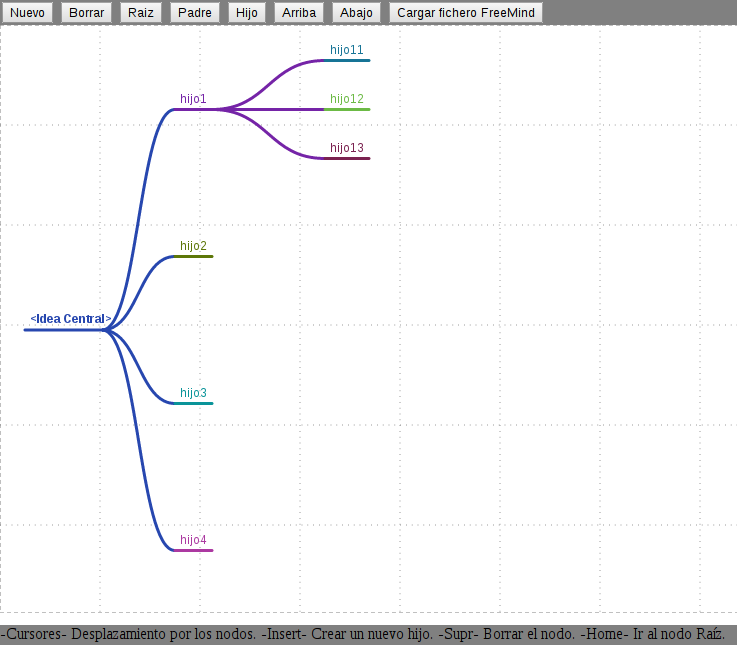
\includegraphics[width=0.5\linewidth]{imagenes/primeraVersion1}
\caption{Versión inicial.}
\label{fig:versioninicial1}
\end{figure}


\begin{itemize}
\item \textbf{Librería base con soporte para herencia.} Esta librería debe tener toda la funcionalidad básica (bindings, curryings, etc) y debe estar muy optimizada ya que el perfecto funcionamiento de la aplicación dependerá en buena medida de ella.

\item \textbf{Librería para manejo de árboles n-arios.} 

\item \textbf{Librería para el manejo de ficheros.} Será la encargada de manejar ficheros, a partir de ella, realizaremos las clases de exportación e importación de mapas mentales de la aplicación. 

\item \textbf{Librería gráfica.} Ciñéndonos al contexto 2D, necesitamos un wrapper sobre la librerías propias del canvas. Esta librería, nos debe permitir pintar, cada uno de los elementos de nuestro árbol. Además de configurar, atributos visuales tales como color del trazo, relleno, etc. No se descarta el uso de alguna librería estándar. Para ello, se realizará una pruebas de concepto sobre ellas.

\item \textbf{Librería para el manejo de eventos del canvas.} El canvas debe reaccionar tanto al teclado, ratón y touch. El canvas viene desprovisto de eventos sobre los elementos pintados en él y es aquí donde entra en juego esta librería. 

\item Por último, las librerías propias del mapa y \textbf{prototipo} o primera versión. 
\end{itemize}

\begin{figure}[tbph]
\centering
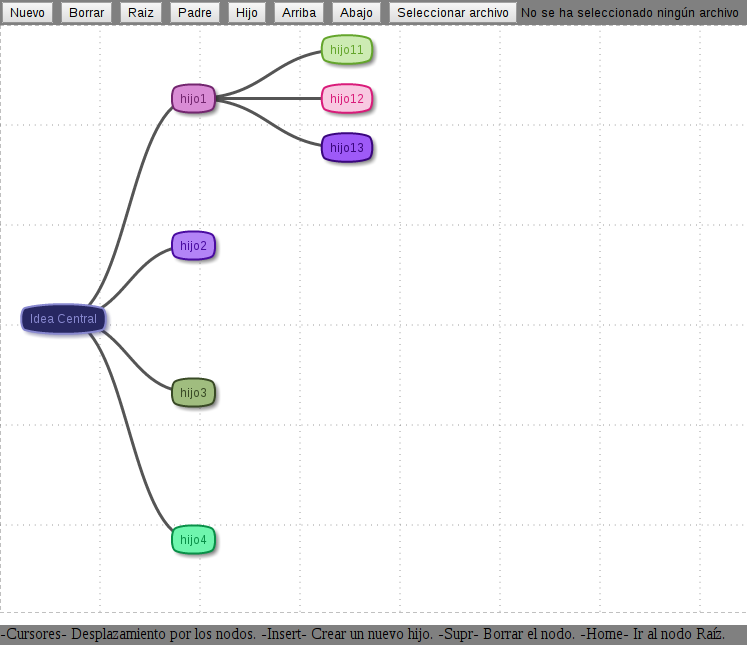
\includegraphics[width=0.5\linewidth]{imagenes/primeraVersion2}
\caption{Versión inicial.}
\label{fig:versioninicial2}
\end{figure}


\textbf{Segunda iteración:} una vez implementadas todas las librerías necesarias y una primera versión (inoperativa), nos encontramos en disposición de ir elaborando la aplicación. Revisión de aspectos visuales de la aplicación tales, como un editor ajustable, zoom, y mejoras en el funcionamiento en general. 

\textbf{Tercera iteración:} nuevas funcionalidades como plegado, hacer-deshacer y un mejor ajuste del en la redistribución de nodos y escalado.


